\chapter{Deuxième Version : Robot Cognitif}


Les robots  cognitifs sont tout d'abord des robots interactifs. La seule différence c'est qu'ils sont dotés de la capacité de se mémoriser la position de la base après l'avoir trouvé. Cette différence sera d'ailleurs la seule que l'on pourra remarquer dans les diagrammes des deux cotés.


\section{Diagramme de Classes}

Le diagramme de classe aussi ne contient pas beaucoup de changements pour les robots cognitifs. En plus du diagramme de classe précédent, nous avons une nouvelle classe "smart\_species" (robot cognitif) qui hérite de la classe "test\_species" (robot réactif) avec un seul nouvel attribut: "la\_base". En effet il contient les coordonnées de la base permettant ainsi au robot de pouvoir s'y diriger directement. La méthode aller\_base() y est redéfinie.

\begin{figure}[!h]
	\begin{center}
		%taille de l'image en largeur
		%remplacer "width" par "height" pour régler la hauteur
		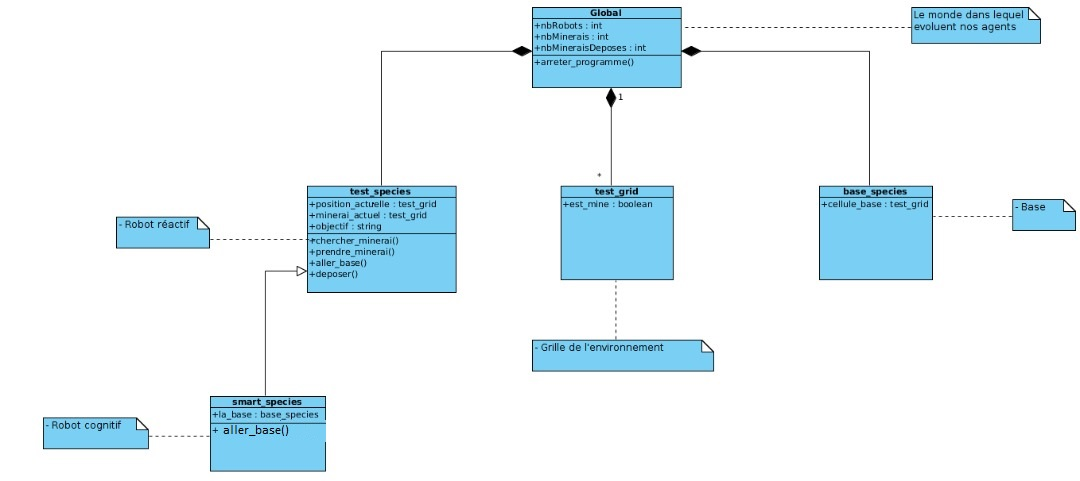
\includegraphics[width=500pt]{diagrammes/diagramme_classe_cognitif}
	\end{center}
	%légende de l'image
	\caption{Réflexe deposer}
\end{figure}

\section{Diagramme d'Activités}

Le diagramme d'activités du Robot Cognitif est le même que celui du robot réactif mis à part le fait que l'activité "Aller à la base" ne se fait pas de la même façon.
\newpage

\subsection{Acheminement des minerais vers la base [Aller a la Base]}

 En effet le déplacement aléatoire ne se fait que lors du premier voyage de transport du minerai vers la base. Après le dépôt le robot sauvegarde les coordonnées de la base pour s'y diriger directement dans le futur. 
 
\begin{figure}[!h]
	\begin{center}
		%taille de l'image en largeur
		%remplacer "width" par "height" pour régler la hauteur
		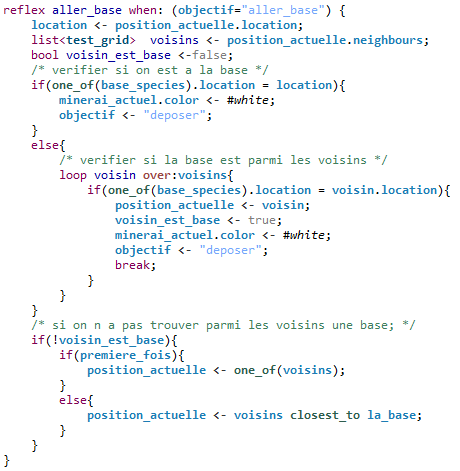
\includegraphics[width=500pt]{code/aller_base_cognitif}
	\end{center}
	%légende de l'image
	\caption{Réflexe aller\_base - Version cognitive}
\end{figure}


